\begin{enumerate}[label=\thechapter.\arabic*,ref=\thechapter.\theenumi]
\item
For the circuit given below, choose the angular frequency $ \omega_0$ at which voltage across capacitor has maximum amplitude?
\begin{figure}[h!]
    \includegraphics[width = 0.5\columnwidth]{2023/BM/16/figs/c_fig1.pdf}
    \caption{circuit }
    \centering
    \label{fig: bm_16_fig_1}
\end{figure}
\begin{enumerate}
    \item[(A)] 1000
    \item[(B)] 100
    \item[(C)] 1
    \item[(D)] 0   
\end{enumerate}
\hfill(GATE BM 2023 Question 16)\\

\solution
\input{2023/BM/16/asnmt3.tex}
\newpage
\item
In the following circuit, the switch S is open for $t < 0$ and closed for $t \ge 0$.
What is the steady state voltage (in Volts) across the capacitor when the switch is closed?
\begin{figure}[h!]
    \includegraphics[width = 0.7\columnwidth]{2023/BM/30/figs/c_fig1.pdf}
    \caption{circuit }
    \centering
    \label{fig:bm_30_fig_1}
\end{figure}
\hfill(GATE BM 2023 Question 30) \\
\solution
\iffalse
\let\negmedspace\undefined
\let\negthickspace\undefined
\documentclass[journal,12pt,twocolumn]{IEEEtran}
\usepackage{cite}
\usepackage{amsmath,amssymb,amsfonts,amsthm}
\usepackage{algorithmic}
\usepackage{graphicx}
\usepackage{textcomp}
\usepackage{xcolor}
\usepackage{txfonts}
\usepackage{listings}
\usepackage{enumitem}
\usepackage{mathtools}
\usepackage{gensymb}
\usepackage{comment}
\usepackage[breaklinks=true]{hyperref}
\usepackage{tkz-euclide}
\usepackage{listings}
\usepackage{gvv}
\def\inputGnumericTable{}
\usepackage[latin1]{inputenc}
\usepackage{color}
\usepackage{array}
\usepackage{longtable}
\usepackage{calc}
\usepackage{multirow}
\usepackage{hhline}
\usepackage{ifthen}
\usepackage{lscape}

\newtheorem{theorem}{Theorem}[section]
\newtheorem{problem}{Problem}
\newtheorem{proposition}{Proposition}[section]
\newtheorem{lemma}{Lemma}[section]
\newtheorem{corollary}[theorem]{Corollary}
\newtheorem{example}{Example}[section]
\newtheorem{definition}[problem]{Definition}
\newcommand{\BEQA}{\begin{eqnarray}}
\newcommand{\EEQA}{\end{eqnarray}}
\newcommand{\define}{\stackrel{\triangle}{=}}
\theoremstyle{remark}
\newtheorem{rem}{Remark}
\begin{document}

\bibliographystyle{IEEEtran}
\vspace{3cm}

\title{GATE 2023 BM 30}
\author{EE23BTECH11007 - Aneesh Kadiyala$^{*}$% <-this % stops a space
}
\maketitle
\newpage
\bigskip

\renewcommand{\thefigure}{\theenumi}
\renewcommand{\thetable}{\theenumi}

\vspace{3cm}
\textbf{Question:} In the following circuit, the switch S is open for $t < 0$ and closed for $t \ge 0$.
What is the steady state voltage (in Volts) across the capacitor when the switch is closed?
\begin{figure}[h!]
    \centering
    \includegraphics[width = \columnwidth]{2023/BM/30/figs/c_fig1.pdf}
\end{figure}
\\
\solution
\\
\fi
\begin{figure}[h!]
    \centering
    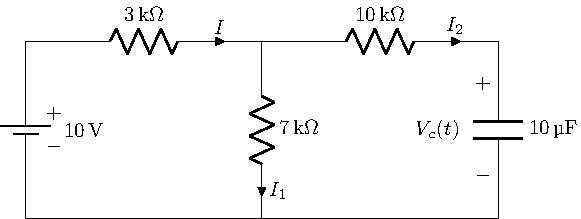
\includegraphics[width=\columnwidth]{2023/BM/30/figs/c_fig3.pdf}
\end{figure}
\\
In steady state, no current flows through the capacitor.
\begin{align}
I_2 &= 0 \\
V_c &= \brak{7\text{k}\ohm}I_1 \\
&= \brak{7\text{k}\ohm}I \\
&= \brak{7\text{k}\ohm}\frac{10\text{V}}{10\text{k}\ohm} \\
\implies V_c &= 7\text{V}
\end{align}
In s-domain:
\begin{figure}[h!]
    \centering
    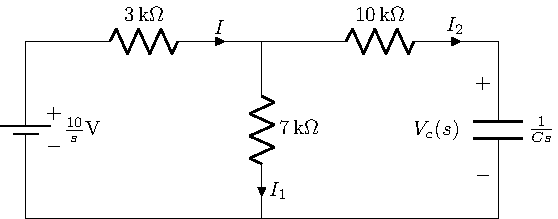
\includegraphics[width=\columnwidth]{2023/BM/30/figs/c_fig2.pdf}
\end{figure}
\begin{align}
\implies I\brak{s} &= \frac{\frac{10}{s}\text{V}}{3\text{k}\ohm + \frac{(7\text{k}\ohm)(10\text{k}\ohm + \frac{1}{sC})}{17\text{k}\ohm + \frac{1}{sC}}} \\
I &= I_1 + I_2 \\
I_1\brak{7\text{k}\ohm} &= I_2\brak{10\text{k}\ohm + \frac{1}{sC}} \\
I_2\brak{s} &= \frac{7\text{k}\ohm}{17\text{k}\ohm + \frac{1}{sC}}I\brak{s} \\
%&= \frac{\frac{70000}{s}}{121 * 10^6 + \frac{10000}{sC}} \\
%&= \frac{\frac{7}{s}}{121 * 10^2 + \frac{1}{sC}} \\
\implies I_2\brak{s} &= \frac{7\brak{10^{-5}}}{0.121s + 1} \\
V_c\brak{s} &= I_2\brak{s}\frac{1}{sC} \\
&= \frac{7}{s\brak{0.121s + 1}} \\
%&= 7\brak{\frac{\frac{1}{0.121}}{s\brak{s + \frac{1}{0.121}}}} \\
&= 7\brak{\frac{1}{s} - \frac{1}{s + \frac{1}{0.121}}}
\end{align}
Taking inverse Laplace transform:
\begin{align}
V_c\brak{t} &= 7u\brak{t}\brak{1 - e^{-\frac{t}{-0.121}}} \label{eq:2023BM30}
\end{align}
\begin{figure}[h!]
\centering
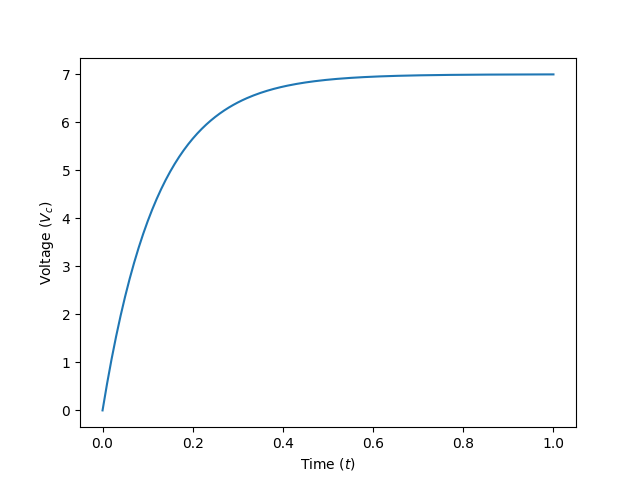
\includegraphics[width=\columnwidth]{2023/BM/30/figs/plot.png}
%\caption{$V_c$ vs $t$}
\label{fig:2023BM30}
\end{figure}
\\
In steady state $t \to \infty$. From \eqref{eq:2023BM30}:
\begin{align}
\lim_{t\to\infty}V_c\brak{t} &= 7\text{V}
\end{align}

\pagebreak
\item 
A finite impulse response (FIR) filter has only two non-zero samples in its impulse response $h[n]$, namely $h[0] = h[1] = 1$. The Discrete Time Fourier Transform (DTFT) of $h[n]$ equals $H(e^{j\omega})$, as a function of the normalized angular frequency $\omega$. For the range $\abs{\omega} \leq \pi$, $\abs{H(e^{j\omega})}$ is equal to
\begin{enumerate}
	\item[(A)] $2\abs{\cos(\omega)}$
	\item[(B)] $2\abs{\sin(\omega)}$
	\item[(C)] $2\abs{\cos(\frac{\omega}{2})}$
	\item[(D)] $2\abs{\sin(\frac{\omega}{2})}$
\end{enumerate}
\hfill(GATE BM 2023 Question 17) \\
\solution
\input{2023/BM/17/1.tex}
\pagebreak
\item
For the circuit shown,if $i=\sin 1000t$, the instantaneous value of the Thevenin's voltage(in volts) across the terminals a anb b at time t=5ms is\\[2pt]

\begin{circuitikz}[american voltages,american currents]
    % Draw the circuit components
    \draw (0,0) -- (2,0);
    \draw (2,2) to [resistor,l=$10\Omega$] (2,4);
    \draw (2,4) -- (0,4);
    \draw (2,0) to [capacitor,l=$-j10\Omega$,-,i_=$i_x$] (2,2);
    \draw (2,0) -- (5,0);
    \draw (5,0) to[inductor,l=$j10\Omega$] (5,2);
    \draw (5,2) to [resistor,l=$10\Omega$] (5,4);
  \draw (5,4) to [cV,l^=$4i_x$,invert] (2,4);
  \draw (5,4) -- (6,4);
  \draw (6,4) to[I,l=$\sin 1000t$,invert] (6,0);
  \draw (6,0) -- (5,0);
   \node[circle,fill=black,inner sep=1.5pt,label=above:a] at (0,0) {};
    \node[circle,fill=black,inner sep=1.5pt,label=above:b] at (0,4) {};
    \end{circuitikz}
    \hfill(GATE EE 2023 ) \\
    \solution
    \input{2023/EE/51/gate51.2023.tex}
    \pagebreak

    \item In the circuit shown ,$\omega=100\pi\text{rads/s}$, R1=R2=$2.2\Omega$ and L=$7\text{mH}$. the capacitance $\text{C}$ for which $Y_{in}$ is purely real is  $\text{mF}$ \\
	\begin{center}
	\begin{circuitikz} \centering \draw 
		(0,4) to[sinusoidal voltage source, l=$V_{0}$cos($\omega$t)] (0,0)
		(0,4) to[short] (4,4)
		(4,4) to[resistor, l=$R_1$ ] (4,2)
		(4,2) to[inductor, l= $\text{L} $] (4,0) to[short ] (0,0)
		(8,4)  to[short] (4,4)
		(8,4) to[resistor, l= $R_2$] (8,2) to[capacitor,l=$\text{C}$] (8,0) to (4,0);
	\end{circuitikz}
	\end{center}
\hfill(GATE IN 2023 Q46)\\
\solution
\input{2023/IN/46/7.tex}

\pagebreak
\item An input voltage in the form of a square wave of frequency $1\, kHz$ is given to a circuit, which results in the output shown schematically below. Which one of the following options is the CORRECT representation of the circuit? \hfill(GATE PH 2023 Q37)
\begin{figure}[!h]
    \centering
    \includegraphics[width = 0.6\columnwidth]{2023/PH/37/figs/question.png}
	\caption{}\
	\label{fig:ques_gate.ph.23.37}
\end{figure}

\begin{enumerate}[label = (\alph*)]
    \item 
    \begin{figure}[!h]
        \centering
	    \resizebox{0.2\textwidth}{!}{\input{2023/PH/37/figs/optA}}
	\label{optA_gate.ph.23.37}
    \end{figure}

    \item 
    \begin{figure}[!h]
        \centering
        \resizebox{0.2\textwidth}{!}{\input{2023/PH/37/figs/optB}}
        \label{optB_gate.ph.23.37}
    \end{figure}

    \item 
    \begin{figure}[!h]
        \centering
        \resizebox{0.2\textwidth}{!}{\input{2023/PH/37/figs/optC}}
        \label{optC_gate.ph.23.37}
    \end{figure}

    \item 
    \begin{figure}[!h]
        \centering
        \resizebox{0.2\textwidth}{!}{\input{2023/PH/37/figs/optD}}
        \label{optD_gate.ph.23.37}
    \end{figure}
\end{enumerate} \hfill(GATE 2023 PH 37)\\
\solution
\input{2023/PH/37/GATE_PH_23_37.tex}
\pagebreak

\item In the circuit shown below, switch S was closed for long time. If the switch is opened at $t=0$, the  maximum magnitude of the voltage $V_R$ , in volts is (rounded off to the nearest integer)\hfill{(GATE 2023 EC 35)}\\
\begin{figure}[h!]
    \centering
    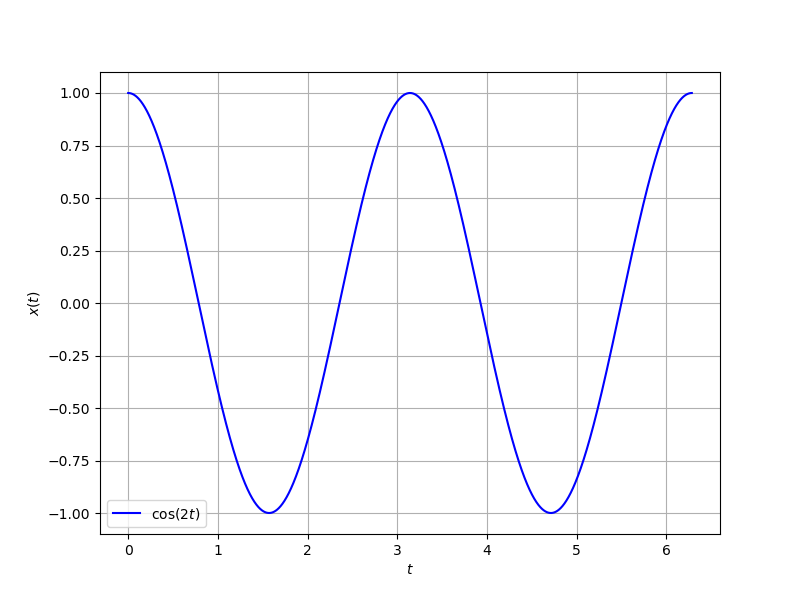
\includegraphics[width=1\linewidth]{2023/EC/35/figs/gate.png}
    \caption{ }
\end{figure}
\solution
\input{2023/EC/35/assign3.tex}
\pagebreak
\item A signal $x\brak{t}=2\cos{(180\pi t)}\cos{(60\pi t)}$ is sampled at 200 Hz and then passed through an ideal low pass filter having cut-off frequency of 100 Hz.\\
The maximum Frequency present in the filtered  signal in Hz is \rule{1cm}{0.5mm} (Round off to the nearest integer.) \hfill (GATE 2023 EE)
\solution
\iffalse
\let\negmedspace\undefined
\let\negthickspace\undefined
\documentclass[journal,12pt,twocolumn]{IEEEtran}
\usepackage{cite}
\usepackage{amsmath,amssymb,amsfonts}
\usepackage{graphicx}
\usepackage{textcomp}
\usepackage{xcolor}
\usepackage{txfonts}
\usepackage{listings}
\usepackage{enumitem}
\usepackage{mathtools}
\usepackage{gensymb}
\usepackage{comment}
\usepackage[breaklinks=true]{hyperref}
\usepackage{tkz-euclide} 
\usepackage{listings}
\usepackage{gvv}                                        
\def\inputGnumericTable{}                                 
\usepackage[latin1]{inputenc}                                
\usepackage{color}                                            
\usepackage{array}                                            
\usepackage{longtable}                                       
\usepackage{calc}                                             
\usepackage{multirow}                                         
\usepackage{hhline}                                           
\usepackage{ifthen}                                           
\usepackage{lscape}
\usepackage[export]{adjustbox}
\usepackage{pgfplots}
\newtheorem{theorem}{Theorem}[section]
\newtheorem{problem}{Problem}
\newtheorem{proposition}{Proposition}[section]
\newtheorem{lemma}{Lemma}[section]
\newtheorem{corollary}[theorem]{Corollary}
\newtheorem{example}{Example}[section]
\newtheorem{definition}[problem]{Definition}
\newcommand{\BEQA}{\begin{eqnarray}}
	\newcommand{\EEQA}{\end{eqnarray}}
\newcommand{\define}{\stackrel{\triangle}{=}}
\newtheorem{rem}{Remark}

\begin{document}
	\parindent 0px
	\bibliographystyle{IEEEtran}
	
	\vspace{3cm}
	
	\title{GATE:EE/63}
	\author{EE23BTECH11208 - Manohar K$^{*}$
	}
	\maketitle
	\newpage
	\bigskip
	
	% \renewcommand{\thefigure}{\theenumi}
	% \renewcommand{\thetable}{\theenumi}
	
	
	
	\textbf{Question:} \hspace{2pt} A signal $x\brak{t}=2\cos{(180\pi t)}\cos{(60\pi t)}$ is sampled at 200 Hz and then passed through an ideal low pass filter having cut-off frequency of 100 Hz.\\
	The maximum Frequency present in the filtered  signal in Hz is \rule{1cm}{0.5mm} (Round off to the nearest integer.) \hfill (GATE 2023 EE)\\
	\noindent \textbf{Solution:}\\
\fi
	\begin{figure}[ht]
		\centering
		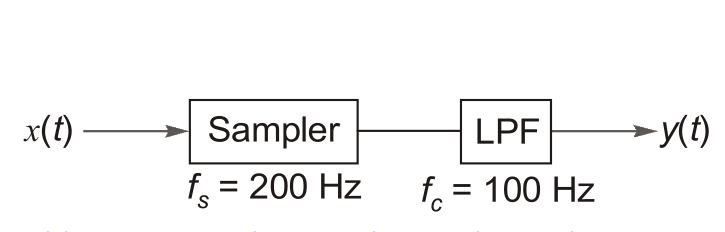
\includegraphics[width=1\linewidth]{2023/EE/63/figs/answerdia.png}
	\end{figure}
	Given, \\
	
	\begin{align}
		x\brak{t}&=\cos\brak{240\pi t} + \cos\brak{120\pi t}
	\end{align}\\
	\begin{table}[h]
		\centering
		
\begin{tabular}{|c|c|c|}
	\hline
	\textbf{symbol} & \textbf{value} & \textbf{description} \\
	\hline
	$x(t)$ & $2\cos{(180\pi t)}\cos{(60\pi t)}$ & input signal \\
	\hline
	$f_s$ & $200Hz$ & sampling frequency \\
	\hline
	$f_c$ & $100Hz$ & cut-off frequency \\
	\hline
	$y(t)$ &  & output signal \\
	\hline
	$f_1$ & $120Hz$ & first signal frequency \\
	\hline
	$f_2$ & $60Hz$ & second signal frequency \\
	\hline
\end{tabular}

		\caption{Parameters}
		\label{tab:GATE.EE.2023.63}
	\end{table}\\
	Aliased frequencies when $f_1$ frequency signal is sampled at $200Hz$\\
	\begin{align}
		& f_1 , \abs{f_s\pm f_1} , \abs{2f_s \pm f_1} \dots\\
		& 120, 80,340,280,520 \dots
	\end{align}
	Aliased frequencies when $f_2$ frequency signal is sampled at $200Hz$\\
	\begin{align}
		& f_2 , \abs{f_s\pm f_2} , \abs{2f_s\pm f_2} \dots\\
		& 60 , 140,260,340,460 \dots 
	\end{align}
\begin{figure}
	\centering
	\begin{tikzpicture}
\begin{axis}[
    axis lines=middle,
    xlabel=$f$,
    ylabel=$X(f)$,
    ymax=1,
    ymin=0,
    xmin=-240,
    xmax=240,
    xtick={ -120, -60, 60, 120},
    ytick={0,1},
    yticklabels={0,1},
    ticklabel style={font=\tiny},
    enlargelimits={abs=0.2},
    clip=false
]
% One-sided arrows
\draw[->, >=latex, blue, thick] (axis cs: -120, 0) -- (axis cs: -120, 1);
\draw[->, >=latex, blue, thick] (axis cs: -60, 0) -- (axis cs: -60, 1);
\draw[->, >=latex, blue, thick] (axis cs: 60, 0) -- (axis cs: 60, 1);
\draw[->, >=latex, blue, thick] (axis cs: 120, 0) -- (axis cs: 120, 1);
\end{axis}
\end{tikzpicture}

	\caption{delta function of input signal }
\end{figure}\\
	
	
\begin{figure}
	\centering
	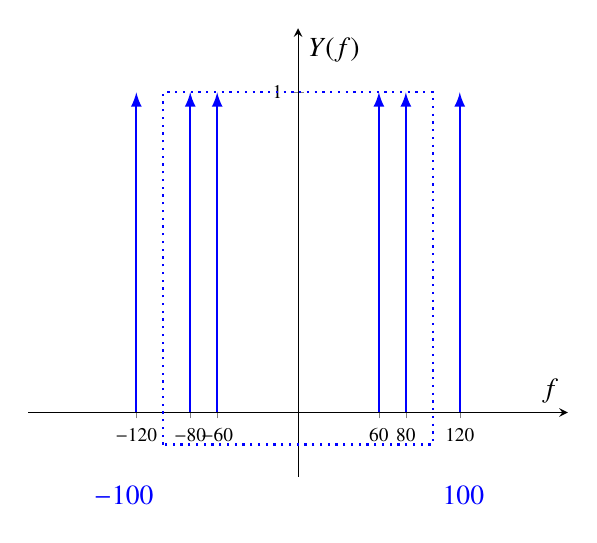
\begin{tikzpicture}
\begin{axis}[
    axis lines=middle,
    xlabel=$f$,
    ylabel=$Y(f)$,
    ymax=1,
    ymin=0,
    xmin=-200,
    xmax=200,
    xtick={ -120, -80, -60, 60, 80, 120},
    ytick={0,1},
    yticklabels={0,1},
    ticklabel style={font=\scriptsize},
    enlargelimits={abs=0.2},
    clip=false
]
% One-sided arrows
\draw[->, >=latex, blue, thick] (axis cs: -120, 0) -- (axis cs: -120, 1);
\draw[->, >=latex, blue, thick] (axis cs: -80, 0) -- (axis cs: -80, 1);
\draw[->, >=latex, blue, thick] (axis cs: -60, 0) -- (axis cs: -60, 1);
\draw[->, >=latex, blue, thick] (axis cs: 60, 0) -- (axis cs: 60, 1);
\draw[->, >=latex, blue, thick] (axis cs: 80, 0) -- (axis cs: 80, 1);
\draw[->, >=latex, blue, thick] (axis cs: 120, 0) -- (axis cs: 120, 1);
% Dotted box
\draw[blue, dotted, thick] (axis cs: -100, -0.1) rectangle (axis cs: 100, 1);
\node[blue, below right] at (axis cs: 100, -0.2) {$100$};
\node[blue, below left] at (axis cs: -100, -0.2) {$-100$};
\end{axis}
\end{tikzpicture}

	\caption{delta function of sampled and filtered signal }
\end{figure}
	from table $f_c = 100Hz$ \\
	LPF output : $60Hz$ , $80Hz$\\
	Maximum Frequency present in the filtered signal is $80Hz$.
	
	
	

\pagebreak
\item In the circuit shown, the input voltage $V_{in} = 100mV$. The switch and the opamp are ideal. At time $t=0$, the intial charge stored in the $10nF$ capacitor is $1nC$, with the polarity as indicated in the figure. The switch $S$ is controlled using a $1KHz$ square-wave voltage signal $V_s$ as shown. Whenever $V_s$ is `High', $S$ is in position $`1$' and when $V_s$ is `Low', $S$ is in position `$2$'.\\
At $t = 20ms$, the magnitude of the voltage $V_o$ will be  \\  
\begin{figure}[ht]
  \centering
    \resizebox{0.55\columnwidth}{!}{\begin{circuitikz}[american]
    \draw (0,0) to[R, l=$10K\Omega$] (2,0) to[L, l=$10mH$] (4,0) to[C, l=$1\mu{F}$] (6,0) -- (6,-1) 
    to[sV, l=$100\cos\brak{\omega_0 t}$] (0,-1) -- (0,0)
    (0,-1) node[circ]{} node[left]{$+$}
    (6,-1) node[circ]{} node[right]{$-$};
\end{circuitikz}
}
\end{figure}
\hfill{(GATE IN 2023)}\\
\solution
\pagebreak

\item The value of parameters of the circuit shown in the figure are $R_1=2\ohm$,$R_2=2\ohm$,$R_3=3\ohm$,$L=10 mH$,$C=100\mu F$. For time \(t<0\), the circuit is at steady state with the switch $ 'K'$ in closed condition. If the switch is opened at $t=0$, the value of the voltage across the inductor \brak{V_L}
 at $t=0^{+}$ in Volts is \rule{2cm}{0.4pt} (Round off to 1 decimal place).
\begin{circuitikz}
    \draw (0,0) to [R, R=$R_3$] (0,2);
    \draw (0,3) to [switch, o-o, name=$K$] (0,2);
    \draw (0,3)-- (0,4);
    \draw (0,4) -- (4,4);
    \draw (3,0) to [american current source, l=$10\,\text{A,}\text{DC}$] (3,4);
    \draw (4,4) to (4,5) to (5,5) to[R, l=$R_1$] (6,5);
    \draw (6,5) to(7,5) to[L, l=$L$] (8,5) to (9,5);
    \draw (4,4)to (4,3)to (5,3) to[R, l=$R_2$] (6,3);
    \draw (6,3)to (7,3) to [C, l=$C$] (8,3) to(9,3);
    \draw (9,5) --(9,3);
    \draw (9,4) -- (10,4);
    \draw (10,4)-- (10,0);
    \draw(10,0)--(0,0);
\end{circuitikz} \hfill (GATE 2023 EE 29Q)
\solution
\pagebreak

\item The op amps in the circuit are ideal. The input signals are $V_{S1} = 3 + 0.10 \sin(300t), \text{V}$ and $V_{S2} = -2 + 0.11 \sin(300t)\, \text{V}$. The average value of the voltage $V_0$ is \underline{\hspace{1cm}} volts (rounded off to two decimal places).
\begin{figure}[ht]
\centering
\resizebox{0.55\columnwidth}{!}{\input{2023/IN/59/figs/gate.circuit.tex}}
\end{figure}
\hfill{(GATE IN 2023)}
\solution
\let\negmedspace\undefined
\let\negthickspace\undefined
\documentclass[journal,12pt,twocolumn]{IEEEtran}
\usepackage{cite}
\usepackage{amsmath,amssymb,amsfonts,amsthm}
\usepackage{algorithmic}
\usepackage{graphicx}
\usepackage{textcomp}
\usepackage{xcolor}
\usepackage{txfonts}
\usepackage{listings}
\usepackage{enumitem}
\usepackage{mathtools}
\usepackage{gensymb}
\usepackage{comment}
\usepackage[breaklinks=true]{hyperref}
\usepackage{tkz-euclide}
\usepackage{listings}
\usepackage{gvv}
\def\inputGnumericTable{}
\usepackage[latin1]{inputenc}
\usepackage{color}
\usepackage{array}
\usepackage{longtable}
\usepackage{calc}
\usepackage{multirow}
\usepackage{hhline}
\usepackage{ifthen}
\usepackage{lscape}
\usepackage{circuitikz}

\newtheorem{theorem}{Theorem}[section]
\newtheorem{problem}{Problem}
\newtheorem{proposition}{Proposition}[section]
\newtheorem{lemma}{Lemma}[section]
\newtheorem{corollary}[theorem]{Corollary}
\newtheorem{example}{Example}[section]
\newtheorem{definition}[problem]{Definition}
\newcommand{\BEQA}{\begin{eqnarray}}
\newcommand{\EEQA}{\end{eqnarray}}
\newcommand{\define}{\stackrel{\triangle}{=}}
\theoremstyle{remark}
\newtheorem{rem}{Remark}
\begin{document}

\bibliographystyle{IEEEtran}
\vspace{3cm}

\title{Gate 2023- Instrumentation Engineering}
\author{EE23BTECH11037 - M Esha$^{*}$% <-this % stops a space
}
\maketitle
\newpage
\bigskip

\renewcommand{\thefigure}{\theenumi}
\renewcommand{\thetable}{\theenumi}

\vspace{3cm}
\textbf{Question 59:} 
The op amps in the circuit are ideal. The input signals are $V_{S1} = 3 + 0.10 \sin(300t), \text{V}$ and $V_{S2} = -2 + 0.11 \sin(300t)\, \text{V}$. The average value of the voltage $V_0$ is \underline{\hspace{1cm}} volts (rounded off to two decimal places).

\begin{figure}[ht]
\centering
\resizebox{0.55\columnwidth}{!}{\begin{circuitikz}

% Lines
\draw (-2.5,2.5) -- (0.5,2.5);
\draw (0.5,3) -- (0.5,1);
\draw (0.5,1.5) -- (0,1.5);
\draw (0,1.5) -- (0,0);
\draw (-2.5,-4) -- (0.5,-4);
\draw (0.5,-4.5) -- (0.5,-2.5);
\draw (0.5,-3) -- (0,-3);
\draw (0,-3) -- (0,-1.5);
\draw (0.5,3) -- (2,2);
\draw (0.5,1) -- (2,2);
\draw (2,2) -- (3.5,2);
\draw (3.5,2) -- (5.5,2);
\draw (3.5,2) -- (3.5,1.5);
\draw (0.5,-2.5) -- (2,-3.5);
\draw (0.5,-4.5) -- (2,-3.5);
\draw (2,-3.5) -- (3.5,-3.5);
\draw (3.5,-3.5) -- (3.5,-3);
\draw (3.5,-3.5) -- (5.5,-3.5);
\draw (5.5,-3.5) -- (5.5,-2.25);
\draw (5.5,2) -- (5.5,0.75);
\draw (5.5,-0.75) -- (6.5,-0.75);
\draw (0,0) -- (3.5,0);
\draw (0,-1.5) -- (3.5,-1.5);
\draw (6.5,-1.5) -- (6.5,-2.5);
\draw (6.25,-2.5) -- (6.75,-2.5);
\draw (6.3,-2.55) -- (6.7,-2.55);


% Resistors
\draw (3.5,1.5) to [resistor] (3.5,0);
\draw (3.5,0) to [resistor] (3.5,-1.5);
\draw (3.5,-1.5) to [resistor] (3.5,-3);
\draw (5.5,0.75) to [resistor] (5.5,-0.75);
\draw (5.5,-0.75) to [resistor] (5.5,-2.25);

% Labels
\node at (-3,2.5) {$V_{S1}$};
\node at (-3,-4) {$V_{S2}$};
\node at (0.75,2.5) {+};
\node at (0.75,1.5) {-};
\node at (0.75,-3) {-};
\node at (0.75,-4) {+};
\node at (7,-0.75) {$V_o$};
\node at (4.25,0.75) {R};
\node at (4.25,-0.75) {R};
\node at (4.25,-2.25) {R};
\node at (6.25,0) {R};
\node at (6.25,-1.5) {R};
\node at (6.75,-0.8) {+};
\node at (6.75,-1.5) {-};

% Dot 
\filldraw (6.5,-0.75) circle [radius=0.05];
\fill (6.5,-1.5) circle [radius=0.05]; 

\end{circuitikz}

}
\end{figure}
\hfill{(GATE IN 2023)}\\
\solution
\begin{table}[h!]
  \centering
  \begin{tabular}{|c|c|c|}
  \hline
  \textbf{Variable} & \textbf{Value} & \textbf{Description} \\
  \hline
  $V_{s1}$ & $3 + 0.10 \sin(300t)$ & \multirow{2}{*}{Input voltages} \\
  \cline{1-2}
  $V_{s2}$ & $-2 + 0.11 \sin(300t)$ & \\
  \cline{1-3}
  $R$ & & Resistances of the resistors \\
  \cline{1-3}
  $V_o$ & & Output voltage \\
  \cline{1-3}
  $V_1$ & & Output voltage of $V_{s1}$ opamp \\
  \cline{1-3}
  $V_2$ & & Output voltage of $V_{s2}$ opamp \\
  \hline
\end{tabular}

  \caption{Input Parameters}
    \label{tab:table1}
\end{table}\\
the current does not flow through op-amp. voltage drop by each R
\begin{align}
&= V_{s1}-V_{s2}
\end{align}
by KVL,
\begin{align}
V_{s2}-V_2&=V_{s1}-V_{s2}\\
V_2&=2V_{s2}-V_{s1}\\
V_1-V_{s1}&=V_{s1}-V_{s2}\\
V_1&= 2V_{s1}-V_{s2}\\
V_o&= \frac{V_1+V_2}{2}\\
&=\frac{V_{s1}+V_{s2}}{2}\\
&=\frac{3+0.10\sin(300t)+{-2}+0.11\sin(300t)}{2}\\
&=0.5+ \frac{0.21\sin(300t)}{2}\\
V_{avg}&=\frac{1}{T} \int_{0}^{T} V(t) \,dt\\
&=\frac{300}{2\pi} \int_{0}^{\frac{2\pi}{300}} \left(0.5 + \frac{0.21 \sin(300t)}{2}\right) \, dt\\
&=0.5
\end{align}
\begin{figure}[b]
    \centering
    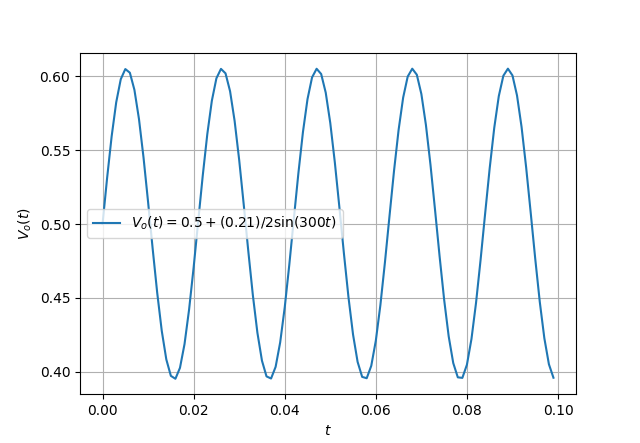
\includegraphics[width=\columnwidth]{59/figs/59fig.png}
    \caption{line plot }
    \label{fig:1}
\end{figure}
\end{document}


\pagebreak

\item The R-L circuit with $R=10 k\Omega$ and $L=1 mH$ is excited by a step current $I_0u(t)$. At $t=0^-$, there is a current $I_L=I_0/5$ flowing through the inductor. The minimum time taken for the current through the inductor to reach $99\%$ of its final value is $\ldots \mu s$
(rounded off to two decimal places).\\
\hfill{(GATE IN 2023)}
\solution
\iffalse
\let\negmedspace\undefined
\let\negthickspace\undefined
\documentclass[journal,12pt,twocolumn]{IEEEtran}
\usepackage{cite}
\usepackage{amsmath,amssymb,amsfonts,amsthm}
\usepackage{algorithmic}
\usepackage{circuitikz}
\usepackage{graphicx}
\usepackage{textcomp}
\usepackage{xcolor}
\usepackage{txfonts}
\usepackage{listings}
\usepackage{enumitem}
\usepackage{mathtools}
\usepackage{gensymb}
\usepackage{comment}
\usepackage[breaklinks=true]{hyperref}
\usepackage{tkz-euclide} 
\usepackage{listings}
\usepackage{gvv}                                        
\def\inputGnumericTable{}                                 
\usepackage[latin1]{inputenc}                                
\usepackage{color}                                            
\usepackage{array}                                            
\usepackage{longtable}                                       
\usepackage{calc}                                             
\usepackage{multirow}                                         
\usepackage{hhline}                                           
\usepackage{ifthen}                                           
\usepackage{lscape}
\newtheorem{theorem}{Theorem}[section]
\newtheorem{problem}{Problem}
\newtheorem{proposition}{Proposition}[section]
\newtheorem{lemma}{Lemma}[section]
\newtheorem{corollary}[theorem]{Corollary}
\newtheorem{example}{Example}[section]
\newtheorem{definition}[problem]{Definition}
\newcommand{\BEQA}{\begin{eqnarray}}
\newcommand{\EEQA}{\end{eqnarray}}
\newcommand{\define}{\stackrel{\triangle}{=}}
\theoremstyle{remark}
\newtheorem{rem}{Remark}
\begin{document}

\bibliographystyle{IEEEtran}
\vspace{3cm}
\title{NCERT Question 11.9.3.9}
\author{EE23BTECH11019 - Faisal Imtiyaz $^{*}$% <-this % stops a space
}
\maketitle
\newpage
\bigskip

\renewcommand{\thefigure}{\arabic{figure}}
\renewcommand{\thetable}{\arabic{table}}


\vspace{3cm}
\textbf{Question:}
The R-L circuit with $R=10 k\Omega$ and $L=1 mH$ is excited by a step current $I_0u(t)$. At $t=0^-$, there is a current $I_L=I_0/5$ flowing through the inductor. The minimum time taken for the current through the inductor to reach $99\%$ of its final value is $\ldots \mu s$
(rounded off to two decimal places).\\
\begin{figure}[h!]
    \centering
    \includegraphics[width=0.8\columnwidth]{question.png}
\end{figure}
\textbf{Solution:}\\
\fi
\begin{tikzpicture}[american]
    % Draw components
    \draw (0,0) to[american current source, l=$I_0$] (0,3); % Current source
    \draw (0,3) -- (2,3) to[R, l=$R$, i=$I_R$] (2,0); % Resistor
    \draw (2,3) -- (4,3) to[L, l=$L$, i=$I_L$] (4,0); % Inductor
    \draw (4,0) -- (0,0); % Connection between resistor and inductor
\end{tikzpicture}

\begin{table}[htbp]
    \centering
    \def\arraystretch{1.5}
    \begin{tabular}{|p{2.5cm}|p{3cm}|}
        \hline
        \textbf{Transform} & \textbf{Signal} \\
        \hline
        $\frac{1}{s(s+a)}$ & $\frac{1}{a}(1-e^{-at})$ \\
        \hline
        $\frac{1}{s+a}$ & $e^{-at}$ \\
        \hline
    \end{tabular}
    \caption{Inverse Laplace transform pairs}
    \label{laplace-transform-pairs-table}
\end{table}

\begin{align}
    I_0u\brak{t} &= I_R + I_L
\end{align}
From KVL, we have:
\begin{align}
    (\frac{I_0}{s} -I_L\brak{s})R - L(sI_L\brak{s} - I_L\brak{0^-}) &=0
\end{align}
After Simplyfying we have:
\begin{align}
    I_L\brak{s} &= \frac{ I_0R +LsI_L\brak{0^-}}{s(R+Ls)}\\
    I_L\brak{s} &= \frac{I_0R}{L}\frac{1}{s(s+\frac{R}{L})} + \frac{I_0}{5}\frac{1}{\frac{R}{L}+s}
\end{align}
From \tabref{laplace-transform-pairs-table}, we have:
\begin{align}
    I_L\brak{t} & = \frac{I_0R}{L} \sbrak{\frac{1}{\frac{R}{L}}(1-e^{-\frac{R}{L}t})} + \frac{I_0}{5}e^{-\frac{R}{L}}\\
    I_L\brak{t} &= I_0 -\frac{4}{5}I_0e^{-\frac{R}{L}t}\\
    I_L\brak{t} &= I_0 -\frac{4}{5}I_0e^{-10^{7}t}\\
    \lim_{t \to \infty} I_L\brak{t} &= I_0
\end{align}
Now time when current in inductor is $99\%$ of its final value is given by:
\begin{align}
    0.99I_0 &= I_0 -\frac{4}{5}I_0e^{-\frac{R}{L}t}\\
    0.01I_0 &= \frac{4}{5}I_0e^{-\frac{R}{L}t}\\
    t &= \frac{L}{R}\ln(80)\\
    t &= 10^{-7}\ln(80) \mu s\\
    t &= 0.43 \mu s
\end{align}
\begin{figure}[ht!]
	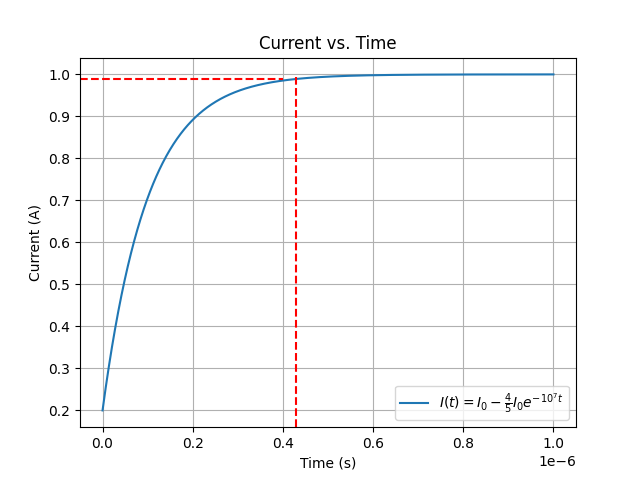
\includegraphics[width=\columnwidth]{2023/IN/47/plots/Figure_1.png}
	% \caption{Plot of $y(n)$ for $a=0.7$}
\end{figure}

  
% \end{document}
\pagebreak


\end{enumerate}
